%% ============================================================
\section{Experiments}\label{sec:experiments}
%% ============================================================

We organize the evaluation around four questions: how much do compositional
inference and aligned training improve verification (RQ1); can CRAFT improve verification
while reducing token use relative to specialized tools (RQ2); do SFT and RL
contribute differently (RQ3); and which design choices enable these gains
(RQ4)?  Appendix~\ref{app:complete-results} collects the complete raw results;
the independent analyses are in Appendix~\ref{app:independent-experiments}.

\subsection{Experimental Setup}
\label{sec:exp:setup}

\tightparagraph{Data and judge.}
Training data comprise 9,024 RL records and 33,346 SFT records (31,865
distinct sources) of target-masked scalar-integer single-loop programs.
The raw training-program pool is drawn primarily from SV-COMP and SyGuS
\citep{svcomp,alur2013sygus}; Appendix~\ref{app:data-curation} describes
program selection and verified SFT-target construction.  SFT
targets and RL rewards are produced only by the open-weight model being trained,
program execution, and Frama-C/WP verification; no external teacher or
closed-model supervision is used.  The
evaluation combines 832 programs from Code2Inv, SyGuS, SV-COMP, LIPuS,
Clause2Inv, and Loopy: 316 linear, 50 nonlinear-arithmetic, and 466 Loopy
instances~\citep{si2020code2inv,alur2013sygus,svcomp,yu2023lipus,
cao2025clause2inv,kamath2023finding}.  No training program matches an
evaluation program under exact, alpha-renamed, or constant-abstracted matching
(Appendix~\ref{app:data-leakage}).  The judge is Frama-C 27.1 (Cobalt) with
the WP plug-in, Typed memory model, and Alt-Ergo/Z3 prover portfolio
~\citep{framac}.  Success requires it to prove induction and every restored
target; all other outcomes count as zero.

\tightparagraph{Inference protocol.}
All \sam{} evaluation runs share target masking, the canonical prompt, clause
processing, Houdini, stochastic decoding, and no re-roll or target feedback;
external tools retain their own target-hidden orchestration.  Each probe curve reuses one
saved pool of \(n_{\mathrm{probe}}\) responses per task.  Appendix~\ref{app:experimental-protocol}
gives decoding, serving, prover, and training details.

\tightparagraph{Metrics.}
Throughout evaluation, success means \(\mathcal G\)-sufficiency under the final
verifier.  pass@\(k\) measures standalone success with a budget of \(k\)
responses; compose@\(k\) measures success after filtering and composing
\(k\) responses.  Displayed pass results use nearest-integer-count projections of reported
rates, including response-pool estimates, while compose evaluates the first \(k\) saved responses.  The two metrics
therefore share a nominal response budget, with different aggregation.
Appendix~\ref{app:experimental-protocol} specifies this distinction and the
reported direct-count results; Appendix~\ref{app:limitations} discusses
sampling variance.


% ---------------------------------------------------------------------------
\subsection{RQ1: How Much Do Compositional Inference and Aligned Training Improve Verification?}
\label{sec:exp:main}

Table~\ref{tab:rcf-paired} compares four local backbones across training
stages, with four API models as references, reporting pass and compose
at one- and eight-response budgets.

% Generated from the current raw-results appendix and cross-model table.
\begin{table}[!t]
\centering
\small
\begin{tabular}{llrrrr}
\toprule
\rowcolor{algobg}
& & \multicolumn{2}{c}{\(k=1\)} & \multicolumn{2}{c}{\(k=8\)} \\
\headercmidrules{\cmidrule(lr){3-4}\cmidrule(lr){5-6}}
\rowcolor{algobg}
\multirow{-2}{*}{Backbone} & \multirow{-2}{*}{Training} & compose & pass & compose & pass \\
\midrule
\multirow{4}{*}{Qwen3-4B}
 & Base & 32.93 & 5.29 & 47.60 & 12.50 \\
 & SFT & 62.62 & 40.38 & 76.20 & 59.98 \\
 & RL & 48.80 & 1.68 & 62.50 & 4.45 \\
 & SFT+RL (\sam{}) & 67.55 & 35.10 & 78.00 & 53.25 \\
\cmidrule(lr){1-6}
\multirow{4}{*}{Qwen3-8B}
 & Base & 37.86 & 6.37 & 54.21 & 17.31 \\
 & SFT & 63.94 & 41.95 & 76.20 & 61.18 \\
 & RL & 51.80 & 2.88 & 64.18 & 7.81 \\
 & SFT+RL (\sam{}) & 69.23 & 36.78 & \textbf{78.73} & 56.49 \\
\cmidrule(lr){1-6}
\multirow{4}{*}{Qwen3-14B}
 & Base & 43.51 & 7.69 & 61.54 & 17.91 \\
 & SFT & 66.35 & \textbf{45.79} & 78.37 & \textbf{63.58} \\
 & RL & 65.38 & 10.34 & 72.24 & 18.63 \\
 & SFT+RL (\sam{}) & \textbf{69.35} & 35.82 & 77.04 & 53.00 \\
\midrule
\multicolumn{6}{l}{\textit{API models}} \\
GPT-5-nano & -- & 33.89 & 3.61 & 55.53 & 16.11 \\
GPT-5 & -- & 51.32 & 32.57 & 72.00 & 51.68 \\
Claude Sonnet-4.6 & -- & 56.97 & 36.30 & 66.95 & 44.95 \\
DeepSeek V4-Flash & -- & 51.44 & 28.13 & 74.40 & 48.20 \\
\bottomrule
\end{tabular}
\caption{Verification across models and training stages (\%). Bold marks each column's maximum.}
\label{tab:rcf-paired}
\end{table}


\tightparagraph{Compositional inference alone substantially improves verification.}
For Bare Qwen3-8B, pass@1 is 6.43\%,
compose@1 reaches 37.86\%, or \(5.89\times\) the standalone rate.
Both rates concern a one-response inference budget, showing that the framework can recover
clauses sufficient for a proof from an answer that fails as a whole.

\tightparagraph{Two-stage training aligned with inference further improves verification.}
SFT constructs supervision from composed valid clause sets, while RL assigns
credit based on the contributions of clauses retained after filtering.
Qwen3-8B compose@1 rises from 37.86\% to 63.90\% after SFT and then to
69.23\% after RL.  All four local backbones show this progressive
improvement in compose@1; Qwen3-4B SFT+RL reaches 67.55\%, exceeding the
highest API reference of 56.97\% under the evaluated protocol.

\begin{insightbox}
\textbf{Finding.}
Compositional inference makes better use of model outputs; supervision and
rewards aligned with that inference process further improve compositional
verification.  Small-model competitiveness comes from the joint effect of
the inference framework and aligned training.
\end{insightbox}

% ---------------------------------------------------------------------------
\Needspace{22\baselineskip}
\subsection{RQ2: Can CRAFT Verify More While Spending Fewer Tokens?}
\label{sec:exp:tools}

\begin{figure}[!t]
\centering
\begin{minipage}[t]{0.333333\textwidth}
\vspace{0pt}
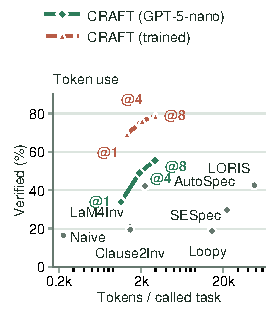
\includegraphics[width=\linewidth]{figures/tool_pareto_row.pdf}
\captionsetup{font=small,margin={0pt,7pt}}
\caption{Verification versus tokens. LLM runs use GPT-5-nano except the local CRAFT cost run.}
\label{fig:tool-pareto}
\end{minipage}%
\begin{minipage}[t]{0.666667\textwidth}
\vspace{0pt}
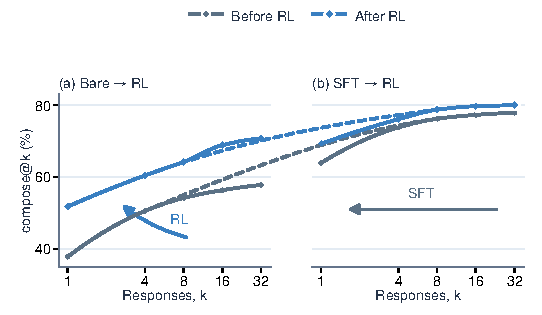
\includegraphics[width=\linewidth]{figures/training_stages_row.pdf}
\captionsetup{font=small,margin={7pt,0pt}}
\caption{Qwen3-8B: RL from (a) Bare and (b) SFT. Solid curves pass through measurements; dashed guides connect interior segments. Arrows illustrate SFT budget compression and RL gains at small \(k\).}
\label{fig:rl-panels}
\end{minipage}
\end{figure}
We compare \sam{} with AutoSpec, SESpec, Clause2Inv, Loopy, and
Daikon~\citep{wen2024enchanting,yang2026sespec,cao2025clause2inv,
kamath2023finding,daikon}, using the same 832-program benchmark and judge.
LLM-based tool comparisons hold GPT-5-nano and target hiding fixed.

\tightparagraph{Clause reuse improves the verification--cost frontier.}
With GPT-5-nano fixed, all three \sam{} budgets lie on the verification--token
Pareto frontier (Figure~\ref{fig:tool-pareto}).  Four responses verify
\textbf{49.04\%} of programs using \textbf{1,905 tokens per task}, exceeding
all compared tools in verification rate while costing less than three of
the four LLM-based baselines.  Eight responses raise verification to
55.53\% at 2,929 tokens.  The locally served trained model reaches 70.31\%
at compose@1; detailed results appear in Appendix~\ref{app:tools-comparison}.

\begin{insightbox}
\textbf{Finding.}
For invariant generation with hidden verification targets and limited
informative feedback, reusable clauses improve the verification--token
trade-off.  Compared with SESpec's iterative repair pipeline, parallel
sampling and composition verify more programs with fewer tokens.
\end{insightbox}

% ---------------------------------------------------------------------------
\subsection{RQ3: How Do SFT and RL Reshape Compositional Search?}
\label{sec:exp:rl}

Prior work suggests that RLVR can increase the sampling frequency of existing
behaviors~\citep{yue2025rlcapacity}.
Figure~\ref{fig:rl-panels} compares Qwen3-8B from Bare and SFT initializations
to examine whether this pattern also appears in compositional verification.

\tightparagraph{SFT expands coverage and compresses the sampling budget.}
SFT reaches 63.90\% compose@1, exceeding Bare compose@32 (57.81\%).
After RL, SFT initialization raises compose@1 from 51.80\% to 69.23\%
under the same one-response budget.
It also raises compose@32 from 57.81\% to 78.37\%: SFT both makes
useful candidates accessible with fewer responses and expands verification
coverage within the measured range.

\tightparagraph{After SFT, RL mainly makes useful candidates available earlier.}
From Bare, RL improves compose@1 and compose@32 by 13.94 and 12.86
points, respectively, retaining a substantial gain even at the largest budget.
After three SFT epochs, its gains shrink to \textbf{5.33 points at compose@1
and only 0.47 at compose@32}.  After SFT, RL mainly improves sampling
efficiency: useful candidates appear with fewer responses, while
coverage at the largest tested budget changes little.

Meanwhile, post-SFT RL lowers pass@1 from 41.93\% to 30.78\%.
The independent clause-cap ablation shows the same trade-off within
SFT+RL: increasing the cap from 4 to 16 lowers standalone response success
while improving compose@1 and compose@8 (Appendix~\ref{app:clause-cap}).  Both results show
that whole-response success can obscure the value of useful clauses within
those responses.

\begin{insightbox}
\textbf{Finding.}
SFT broadens verification coverage and compresses compositional search into
fewer responses.  Post-SFT RL mainly improves sampling efficiency, making
useful candidates available earlier even after substantial supervised training.
\end{insightbox}

% ---------------------------------------------------------------------------
\subsection{RQ4: Why Do Composed SFT Targets and Clause-Level Rewards Help?}
\label{sec:exp:ablations}

\begin{figure}[H]
\centering
\begin{minipage}[t]{0.333333\textwidth}
\vspace{0pt}
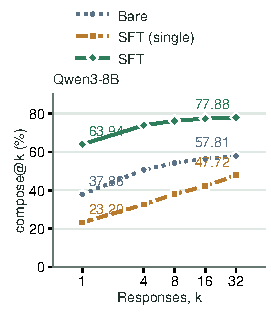
\includegraphics[width=\linewidth]{figures/sft_composition_compose_row.pdf}
\captionsetup{font=small,margin={0pt,7pt}}
\caption{Qwen3-8B SFT targets and compose@\(k\). Labels mark @1 and @32.}
\label{fig:sft-composition-compose}
\end{minipage}%
\begin{minipage}[t]{0.666667\textwidth}
\vspace{0pt}
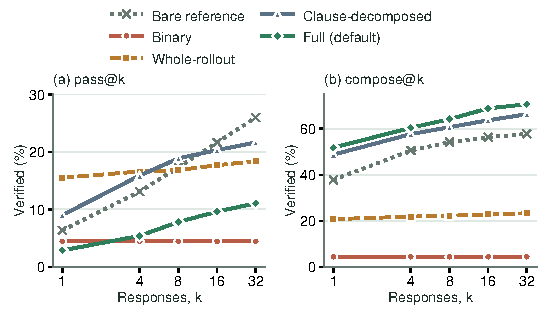
\includegraphics[width=\linewidth]{figures/reward_ablation_row.pdf}
\captionsetup{font=small,margin={7pt,0pt}}
\caption{Qwen3-8B rewards from Bare: (a) pass@\(k\); (b) compose@\(k\). Panels use different y-axis ranges; parentheses mark the default.}
\label{fig:reward-ablation}
\end{minipage}
\end{figure}

We ablate SFT target construction and RL credit assignment to examine how
training acquires useful clauses and preserves their contributions.

\tightparagraph{Composition turns broader exploration into supervision.}
SFT (single) uses independently filtered responses; composed targets pool
valid clauses across responses, giving supervision access to more candidate
invariants and complementary constraints.  With approximately equal numbers
of training examples, composed-target SFT raises Qwen3-8B pass@1 from
19.95\% to 41.93\% and compose@1 from 23.20\% to 63.90\%, relative to
SFT (single) (Figure~\ref{fig:sft-composition-compose}).  Composition exposes
SFT to the results of multi-response exploration, which the trained model
can exploit with a single response.

\tightparagraph{One rejected clause should not erase the others' credit.}
With verification targets hidden, RL uses inductiveness and negative coverage
(Figure~\ref{fig:reward-ablation}).  Binary alone reaches only 4.55\%
compose@32.  Whole-rollout adds coverage but gates credit on the entire
response: pass@1 improves to 15.50\%, yet compose@32 falls to 23.32\%,
below Bare's 57.81\%.  One rejected clause therefore withholds credit from
every useful survivor.  Clause-decomposed removes this gate and reaches
66.35\% compose@32; after SFT, its compose@1 advantage over Whole-rollout
remains 24.28 points.

\tightparagraph{Group credit adds most from Bare.}
Full adds Shapley credit with weight 0.3.  From Bare, it raises compose@32
from 66.35\% to 70.67\%; after SFT, the selected Full model reaches
69.23\% compose@1 versus Clause-decomposed's 67.91\%, while compose@32 improves by only
0.12 points.  The full comparison is in Appendix~\ref{app:full-credit-analysis}.

\label{sec:exp:probe}
Appendix~\ref{app:independent-experiments} reports the complete ablations,
including inference, clause cap, negative sampling, filtering order,
and target visibility.

\begin{insightbox}
\textbf{Finding.}
Composed targets turn useful clauses from broader exploration into supervision;
clause-level rewards preserve useful contributions within failed responses.
Together, they let training exploit more of the candidates that compositional
verification can use.
\end{insightbox}
